%!TEX root = uist14.tex
\section{Iteration 3: Head motion refinement}
\label{sec:iteration-3:-head}
\subsection{Problem Statement and Goal}
Both {\em Naive IR} and {\em Intensity IR} rely on list navigation on the near-eye display for the refinement step. This has two problems: First, a spatial layout of targets is compressed into a uni-dimensional list. List navigation commands thus have poor spatial mapping. Second, our techniques require the user to switch their focus back and forth between the physical world and the display. These issues motivated us to design an approach that also utilizes orientation information during the {\em refinement} stage, to provide a more direct mapping between the user's actions and target selection.

In our third iteration, we ask the question ``can we build a system which further minimize the chance of falling back to list based refinement?''

\subsection{Technique}
The motion sensors (including gyroscope, magnetometer and accelerometer) on the head-worn device can help us determine the orientation of a user's head. However, this absolute orientation cannot be directly used in any indoor environment as the user may change their location. However, as long as the targets are spread around the periphery, their relative orientation to each other is relatively stable (see Figure~\ref{fig:third_principle}). This key observation inspires us to investigate a hybrid solution with IR and orientation sensors on Glass.

\begin{figure}[t]
\centering
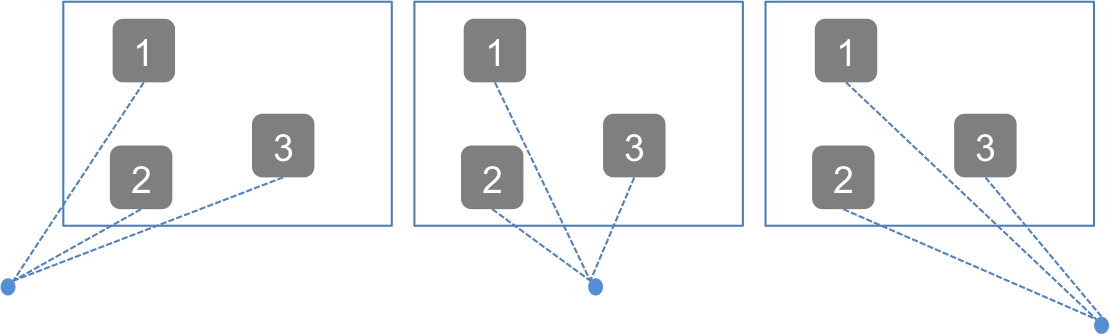
\includegraphics[width=1\columnwidth]{figures/third_principle.png}
\caption{Even when the user's absolution position changes, the relative relationship in the orientation space remain invariant.}
\label{fig:third_principle}
\end{figure}

\begin{figure}[t]
\centering
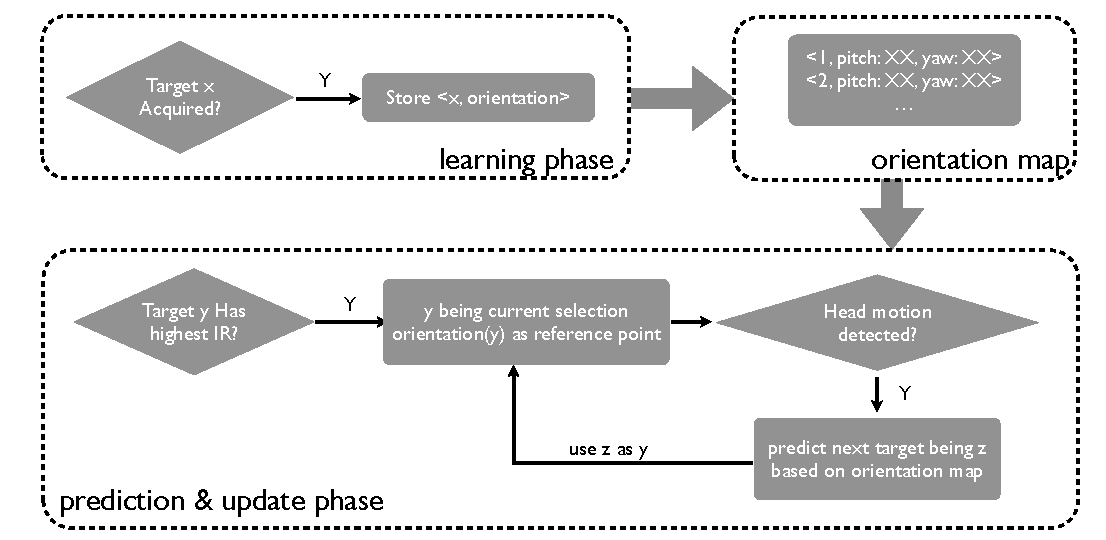
\includegraphics[width=1\columnwidth]{figures/third_technique3.pdf}
\caption{\ben{figure in interactionModel2.key file.} Our third technique learned each target's absolute orientation and construct the orientation map. Though we store the absolute orientation value, during the {\em refinement} stage, the prediction is only based on relative changes to a reference point. In such a way, the prediction will work regardless of user's position.}
\label{fig:third_technique}
\end{figure}

There are two phases to this technique: learning the relative orientations or targets in a room and intelligently suggesting targets during refinement (see Figure~\ref{fig:third_technique}).

In the first stage, the user orients their head towards each device, and the system learns a map of the devices based on their corresponding sensor readings. During the second stage, when the user wishes to use head-motion for disambiguation, they will put their finger on the touchpad to enter a quasi-mode in which their head movement is used to select targets. In this mode, only one device has a solid indicator light on at a time. \bjoern{revisit prior sentence - there's a problem in the current technique in that the user doesn't know which targets are in the refinement set and which aren't.} \achal{There is no longer a refinement set - instead the user can select between all the devices using just orientation once they enter quasi mode.} The user can then tilt in the direction of the device they wish to switch to. This gesture is inspired by observing users who tend to adjust their glasses for closer inspection.

The technical implementation of this interaction involves a number of subtleties due to the noisiness of our data. Absolute orientations between devices change frequently at the slightest user movement, and motion sensor data is inherently noisy. To alleviate the second issue, a low-pass filter is applied to the measurements, allowing us to extract the direction of motion from this smoothed history. Empirically, we found that we can reliably detect the direction of movement with 100ms of history and a sensor resolution of 10ms.

Orientation changes can be overcome by using a hybrid of absolute and relative orientations augmented by IR information. While absolute orientations are unstable, relative orientations do not contain information for essential tasks, such as adding devices to a learned map. Our system stores the absolute orientations of each device during the learning stage, but utilizes only the relative information embedded in this data for disambiguation. Once the user is in quasi-mode, our system calculates the user's direction of motion as described earlier, and searches through the map for the nearest device in that direction. Thus, although the absolute orientation of the currently lit device may be incorrect, the relative information can still be used for disambiguation. Finally, the system uses hysteresis to prevent the user from accidentally jumping repeatedly between devices by switching devices only once the user has moved beyond a certain threshold in any direction. \achal{I understand hysteresis, but I can't figure out how the word can be used naturally (as there's no way to say a system "has" hysteresis). This last sentence may require rewording.}

\bjoern{how well will this work if the user shifts position within a room?}
\achal{I think the updates should explain this now.}

\achal{Not sure if there should be a conclusion of some sort here.}

\subsection{Evaluation}
\ben{We then need evaluation results here, quantitative and qualitative.}
\bjoern{got to here in my pass}


% %!TEX root = uist14.tex
% \section{Iteration 3: Orientation-based refinement}
% \bjoern{While taking IR intensity into account further reduced the need for manual refinement and increased performance, the UI navigation scheme is problematic - it is not spatially related in any meaningful way to the layout of targets in a room. A better interaction technique would respect that ordering. For example, when refinement is needed, tilting the head slightly to the right could select the target that's adjacent to the right of the currently selected target.

% Such spatial navigation requires knowledge about the layout of targets in the environment. However, one of the strengths of our technique so far is that it does not require any map ahead of time. To enable some spatial navigation, we introduce a final iteration in which we build up a spatial data structure by demonstration (i.e., the user looks around the room) and then leverage that data structure during the refinement step of our interaction.}

% \bjoern{This technique is based on the assumption that users will generally select targets in indoor environments where targets are spread around the periphery. These assumptions enable us to use orientation data without knowing the user's absolute position.}

% \subsection{Implementation}
% \bjoern{give implementation details}

% \subsection{Informal User Feedback}
% \bjoern{We informally evaluate this technique with N users: ...}

 
%%% Local Variables: 
%%% mode: latex
%%% TeX-master: "uist14"
%%% End: 
